\documentclass[../main.tex]{subfiles}

\subsection{Feladat}

Készítsünk programot, amellyel a következő két személyes játékot lehet játszani. Adott egy nxn mezőből álló tábla, ahol egy menekülő és egy támadó játékos helyezkedik el. Kezdetben a menekülő játékos figurája középen van, míg a támadó figurái a négy sarokban helyezkednek el. A játékosok felváltva lépnek. A figurák vízszintesen, illetve függőlegesen mozoghatnak 1-1 mezőt, de egymásra nem léphetnek. A támadó játékos célja, hogy adott lépésszámon (4𝑛) belül bekerítse a menekülő figurát, azaz a menekülő ne tudjon lépni.A program biztosítson lehetőséget új játék kezdésére a táblaméret (3x3,5x5, 7x7) és így a lépésszám (12, 20, 28) megadásával, folyamatosan jelenítse meg a lépések számát, valamint az aktuális játék mentésére és egy korábban elmentett játék betöltésére. Ismerje fel, ha vége a játéknak, és jelenítse meg, melyik játékos győzött, illetve azt is, ha döntetlen lett a vége, majd automatikusan kezdjen új játékot.

\subsection{Elemzés}

A játékot két személy játssza, azonban a játék szempontjából csak váltakozó lépések vannak.
Minden játék lépését a vadász fél kezdi, ezzel is növelve a bekerítés esélyét a nagyobb táblákon.
Esetdiagramm nézőpontjából az egyféle játékos az alábbi cselekedeteket végezhet:



\begin{center}
    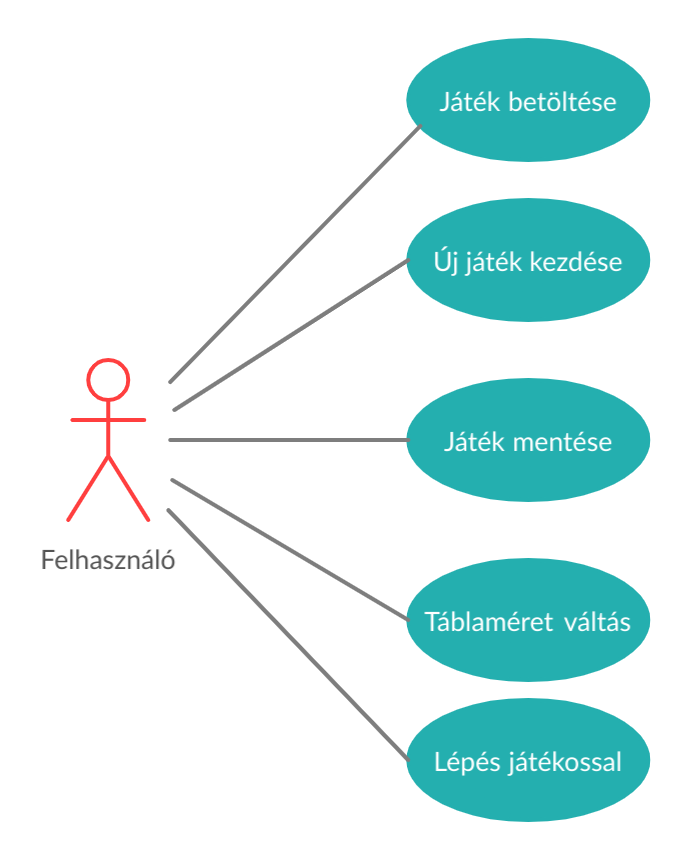
\includegraphics[width= 0.35\textwidth ]{HuntingUseCases.png}
\end{center}
    